% !TEX root = ../main.tex

\chapter{Background}
This chapter introduces to bitcoin, the world of cryptocurrency and marketplaces. It describes as well 
what is a proof of solvency, and some of its evolution and current state.

\section{Bitcoin}

Bitcoin is recognized as the world's first successful cryptocurrency and decentralized digital currency. 
The goal of Bitcoin is to allow financial transactions to be settled without the need of a financial institution.
Transactions can occur within 2 participants of the network in realtime, without any middleman. 
All transactions are settled on a public blockchain, which means that everything can be verified by everyone. 


\subsection{Transactions}
For every participant of the network, there is a public key,  a private key and a wallet address.
The public key is derived from the private key using elliptic curve multiplication, and the wallet address is derived from the public key using a hashing function.
Both are one way function, meaning you cannot derived the other way around.
The wallet address can be sean as a bank account number. When you send bitcoin to someone, you send it to their wallet address.
To be able to send some bitcoin, you need to sign your transaction. 
Since transactions are sent on the network, we need to make sure a transaction originates from the sender.
The way to do that is to sign your transaction. The digital signature is created from the transaction data and the private key, which is only known by the owner of the address.
The public key is then used to make sure that the signature originates from the right private key.
Sending a transaction is the easiest problem to solve. The real challenge is to keep track of who owns what, and to avoid the double spending problem.
The way to do that is to keep the history of every single transactions. 
Bitcoin is a blockchain. The blockchain is made of blocks, and the transactions are filling these blocks.


\subsection{Network}
The challenge of the network, is to have every single node agree on the transaction history. Nodes are computers connected to the network,
working on publishing new blocks. The nodes work together to agree on the order of transactions. Every new transaction is broadcaseed to all nodes.
The nodes puts the transactions into a block, and try to publish that block. In order to publish a block, each node need to solve a proof-of-work challenge.
When a node solves the challenge, it broadcasts the block to every nodes. The nodes accepts the block if all transactions are valid. Their is no formal
way of approving a new block. A node show its acceptance by starting to work on a new block using the hash of the accepted block as previous hash.
Some nodes might accept different blocks, depending on what time they received new blocks. To solve the issue of multiple chains, the longest chain is consideredto be the correct one. 
If two chains have the same length, nodes keep working on their respective chains untill one of the chains receive a new block, breaking the tie.


\subsection{Proof-of-work}
In order to submit a new block, a node have to find a hash with x number of leading 0 bits.
It is exponentially more difficult every time you add a zero. The way to have different hash values, is to change the block timestamp, and the nonce value.
The nonce value is there solely for that purpose. Once a block is published, you cannot change any value inside of it because the hash value would change.
You would need to redo all the work to find a new good hash. Older blocks are even more secured, because in order to change the 2nd to last block, you would need to redo the work
for the 2 latest blocks. This is the same for every block down the road. The longest chanin is determined by the greatest proof-of-work invest in it. If their is a majority of honest nodes,
that chain will grow up the fastest. The difficulty of the new block is determined by an average, in order to generate blocks at a steady pace.


\subsection{Merkle Tree}
Only the merkle root is stored in the block header. When a block is enough in the past, nodes start to only keep block headers in memory.
They do not keep the rest of the block. This is why the hash of a block is the hash of the block header, and not the whole block. To keep the integrity of the chain.
The merkle root is the top of the Merkle Tree. A merkle tree is a tree where the parent node is the hash of the child nodes.

%\bigskip % Add an empty line
%These are optional parameters to finetune the placement of tables and figures, with the following meaning:
%
%h, here
%t, top
%b, bottom
%p, page of float
%e.g. \begin{figure}[!htb]
\begin{figure}[ht!]
\centering
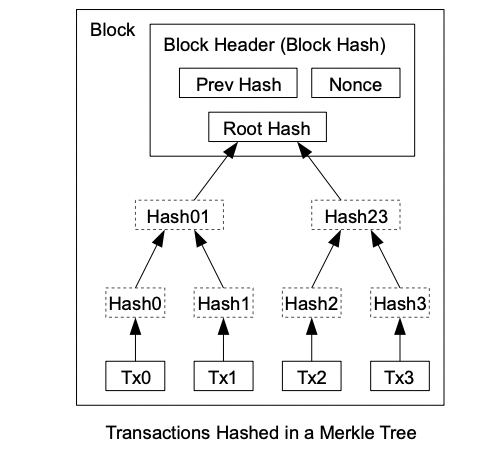
\includegraphics[width=90mm]{MerkleTree.png}
\caption{Bitcoin Merkle Tree \cite{N08}}
\label{overflow}
\end{figure}


%Andreas M. Antonopoulos
%whitepaper
%add figure of merkle tree, bitcoin block, 

%    \item A decentralized peer-to-peer newtork (the bitcoin protocol)
    
%    \item A public transaction ledger (the blockchain)
    
%    \item A set of rules for independent transaction validation and currency issuance (consensus rules) 

%    \item A mechanism for reaching global decentralized concensus on the valid blockchain (Proof-of-Work algorithm)
    
%    \end{enumerate}


%\section{Cryptocurrency}

\section{Marketplaces}

\section{Zero Knowledge}

\section{Proof of solvency}


 
% = = = = = = = = = = = = = = = = = = = = = = = = = = = = = = = = = = = = = = = = = =

\paragraph{Scope.} 
Blah blah blah.

% = = = = = = = = = = = = = = = = = = = = = = = = = = = = = = = = = = = = = = = = = =



